\subsubsection{Referencespænding}
Der skal ved offset- og komparatorblokken forsynes med en konstant spænding, da spændingen skal anvendes som sammenligningsgrundlag ift. andre signaler. Denne spænding kaldes en referencespænding. Referencespændingen består af en spændingsforsyning, en modstand og en spændingsreference diode. Der anvendes en referencediode af typen LM385, som både findes som $1.2$V og $2.5$V. Et eksempel på en opsætning af en spændingsreference kan ses på figur \figref{fig:Spaendingsreference}.

\begin{figure}[H]
	\centering
	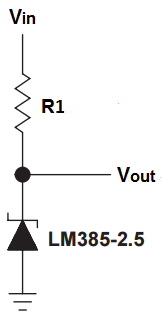
\includegraphics[scale=1.0]{figures/cProblemloesning/ReferenceEksempel}
	\caption{Figuren illustrerer et eksempel på opsætning af et kredsløb for en spændingsreference med LM$385$. Figuren er en revideret udgave fra kilden. \cite{Instruments2005}}
	\label{fig:Spaendingsreference}
\end{figure}

For at udregne værdien af modstanden, R, i kredsløbet, anvendes følgende generelle formel:
\begin{equation}
R=\dfrac{V_{forsyning}-V_{Reference}}{I_{Z}}
\end{equation}
Hvor V_{forsyning} er forsyningsspændingen som sendes ind i kredsløbet, V_{Reference} er den referencespænding der skal sendes ud af systemet og I_{Z} er strøm forbruget fra de komponenter, der er i referencespændings kredsløbet. 
\noindet \textbf{Beregning af referenceværdien til offset}
Først udregnes R for referencespændingen til offsettet. V_{forsyning} er de $5.5$V, der forsynes med fra spændingsforsyningen. V_{Reference} $2.5$V. I kredsløbet for ofsettet indgår én operationsforstærker(TL$081$), der har en maksimal biasstrøm på $200$pA\cite{Corporation1995}. Referencedioden har et arbejdsområde mellem $20\muA$ til $20mA$ og for at sikre der er strøm nok til referencedioden er den sat til at bruge $100\muA$\cite{Instruments2005}. Dermed kan strømforbruget, I_Z, for offsettet udregnes som summen af de to biasstrømme og alle de kendte værdier indsættes i formlen:

\begin{equation}
R_{offset}=\frac{5.5V-2.5V}{0.0001000002A}=29999.94\Omega \approx 30K\Omega
\end{equation}  
Da offsettet på accelerometeret er på $1.6325$V jævnført \ref{Offset_Teori_Design} på side \pageref{Offset_Teori_Design} skal referenceværdi være ligeledes $1.6325$V. For at opnå denne referenceværdi, bruges der en spændingsdeler. Den genelle formel for spændingsdeler er: 

\begin{equation} \label{Spaendingsdeler}
V_{out}=V_{in}*\dfrac{R2}{R1+R2}
\end{equation}

R$1$ bliver valgt til at være $10$K\Omega og derved er følgende kendt: 
\begin{itemize}
\item V_{out}  = $1.6325$V
\item V_{in} = $5.5$V
\item R1 = $10$K\Omega
\end{itemize}
Ligningen kommer til at være således: 
\begin{equation}
1.6325V = 5.5* \dfrac{R2}{10000\Omega+R2} 
R2 = 18818.44380\Omega \approx 18820\Omega
\end{equation}

\noindet \textbf{Beregning af referenceværdien til komparator}
Den samme fremgangsmåde anvendes til udregning af R for referencespændingen til komparatoren. Her er den ønskede referenceværdi  $2.5$V, så der benyttes ikke en spændingsdeler. Der er i begyndelse at kredsløbet indsat en operations forstærker (TL$082$), som har to input og output og derved kan fungere som både buffer til komparator kredsløbet og inverterende forstærker. Da spændingsdeleren går direkte ind i en buffer, så er den maksimale biasstrøm på $50nA$. Biasstrømmen for referencedioden er igen sat til $100\muA$. Dermed kan værdierne igen indsættes i formlen og R kan beregnes.

\begin{equation}
R_komparator=\frac{5.5V-2.5V}{0.000100005A}=29998.50007\Omega \approx 30K\Omega 
\end{equation} 

\textbf{Test af referencespænding}

 